We begin by sketching the architecture of SDN networks and
describing the correctness challenges encountered by operators and
implementers of SDN control platforms. We place particular emphasis on the
properties of SDN that make it suitable for automated diagnosis.

SDN networks are managed by software running on a set of network-attached
servers called `controllers'. It is the job of the controllers to configure
the network in a way that complies with the intentions of network
operators. Operators codify their intentions by configuring
behavioral specifications we refer to as `policies'. Policy constraints might
include connectivity, access control,
resource allocations, traffic engineering objectives, or middlebox
processing.

For fault-tolerance, production SDN control software is typically
distributed across multiple control servers. For scalability, the responsibility for
managing the network can be partitioned through sharding.
Onix~\cite{onix}, for example, partitions a
graph of the network state across either an eventually-consistent
distributed-hash table or a
transactional database.
%allowing control applications to make their own
%tradeoffs in choosing consistency models and degree of fault tolerance.

In this distributed setting, controllers must coordinate among themselves
when reacting to changes from below (state changes in the network), or
changes from above (policy).
Coordination in SDN is not exempt from the well-known class of faults
inherent to all distributed systems, such as
inconsistent reads, race conditions over message arrivals, and
unintended consequences of failover logic.

Several production SDN controllers support network
virtualization~\cite{bigswitch,nicirahomepage,contextream}, a technology that
abstracts the details of the underlying physical network and presents a
simplified view of the network to be configured by applications.
A common pattern is to treat an entire network (up to
100,000 v-switches in a large datacenter) as a single logical switch.
In this model, multi-tenancy is implemented by providing each tenant with their
own abstract view, which are multiplexed onto the same physical network.
When an entire datacenter network is
abstracted into a single logical switch in this way, the mapping between
the logical switch and the physical topology is highly complex.

In conjunction, the challenges of maintaining virtualized and distributed
objects while ensuring that critical invariants such as isolation between
tenants are upheld at all times makes the task of constructing
SDN control software highly complex. Ultimately, complexity brings with it
bugs, and much of developers' time is spent troubleshooting; a commonly cited
number in the software-engineering community is that
developers spend over 50\% of their time
debugging~\cite{msoft_concurrency}. \colin{Cite Nikhil's survey of network
operators, re: troubleshooting}

Luckily, SDN has several properties that make it particularly amenable to an
automated troubleshooting approach such as ours. Most importantly, SDN control software
quickly converges to quiescence--that is, SDN controllers become idle when no policy or
topology changes occur for a period of time. In contrast to long-running iterative computations,
this means that individual inputs to the system have a relatively isolated effect on the outcome
of the computation; if we prune one input from the log and replay the execution, it is unlikely
that the new outcome will be able radically different from the original. If this were not the case, our
technique would not be able to significantly decrease the size of execution traces, as will will become clear in
\S\ref{subsec:algorithm}.

SDN's architecture also facilitates the implementation of our troubleshooting
tool. The syntax and semantics of interfaces between components of the system (\eg~OpenFlow
between controllers and switches~\cite{openflow}, or
OpenStack Quantum's API between
the control application and the network hypervisor~\cite{quantum}), are
well-defined--a property that is crucial for
enabling us to compare altered histories (described in \S\ref{subsec:replay}).
Moreover, controllers are relatively small in number compared to the size of
overall network, which makes it much easier to superimpose
on messages (described in detail in~\S\ref{sec:architecture}).

\subsection{Non-Goals}
\label{subsec:non_goals}

Before diving into the
details, we clarify the scope of our tool's use.

\noindent{\bf Troubleshooting vs Debugging.} Our technique is a troubleshooting tool, not a debugger;
by this we mean that \simulator{} helps identify and localize inputs that
trigger erroneous behavior, but it does not directly identify exactly which
line(s) of code cause the error.

\noindent{\bf Bugs Outside the Control Software.} Our goal is not to find the root
cause of individual component failures in the system; we're only interested in
errors in the way the control software consequently behaves.
Consider a mud slide that causes (i) a network uplink to fail, which subsequently
causes (ii) a switch to overheat and crash. Our
system is agnostic to (ii)'s causal dependence on (i). Instead, we focus on
how the distributed system as a whole reacts to the occurrence of (i) and/or (ii).
If there is a bug in your switch, you should contact your hardware vendor;
if you have a bug in your policy specification, you should take a closer look at what you specified.
That said, our tool can show whether switches behave the same as our software
implementation; if our tool was unable to reproduce the error, that means that
the problem was above or below the control software.

\noindent{\bf Non-determinism Within Individual Controllers.} Our tool is not designed to reproduce bugs
involving non-determinism within a single controller (\eg~race-conditions between threads);
we focus on coarser granularity errors (\eg~incorrect failover logic), which we find plenty of
in \S\ref{subsec:case_studies}.
That said, if the developer is willing to instrument their system to
provide finer granularity log messages (\cf~\cite{Geels:2006:RDD:1267359.1267386}),
our approach readily supports deterministic replay.

\noindent{\bf Globally vs Locally Minimal Input Sequences.}
Delta debugging is not guaranteed to find the globally minimal
causal sequence from an input trace, since this requires $O(2^N)$ computation in the worst case.
Delta debugging is however guaranteed to find a 1-minimal (locally minimal) causal sequence,
meaning that if any input from the sequence is pruned, no correctness violation
occurs~\cite{Zeller:2002:SIF:506201.506206}. \scott{Modify: with single event
order}

\noindent{\bf Correctness vs Performance.}
We are primarily focused on correctness bugs, not performance bugs. That said,
our approach is largely agnostic to what kinds of invariants are
checked~\ref{subsec:cc}.

\noindent{\bf Proactive vs Reactive Configuration.} We focus primarily on
\emph{proactive} configuration, where controllers react to policy and topology changes, but
 not necessarily individual packets or flows events in the dataplane.
Production controllers typically adopt this model for performance reasons~\cite{nicira}.



%--------------------------------------------------------------------%
%               OLD HOTNETS TEXT
\eat{

% Peter: useful to state your assumptions:
%is correct: policies, logical layer specification, physical layer model
%is possibly buggy: logical -> physical layer

We begin by sketching the architecture of SDN networks and
describing the failure-modes and correctness challenges encountered by operators and
implementers of SDN control platforms.

SDN networks are managed by software running on a set of network-attached
servers called ``controllers''. Modern SDN platforms differ from
`first-generation' controllers such as NOX~\cite{nox} in two aspects: they
maintain a virtualized view on top of which control
logic resides, and they distribute state across
multiple control servers.

%Two common patterns of control are proactive and
%reactive. Proactive controllers pre-compute forwarding tables for the entire
%network, and only push down updates periodically to react to link failures,
%changes in traffic mix, \etc. In contrast, in \emph{reactive} SDNs, the
%controller updates the forwarding state in reaction to a \emph{dataplane event},
%e.g., a previously unmatched patched found on the wire.

%Production SDN deployments are commonly proactive, primarily due to the large
%scale of datacenter networks and the current capabilities of forwarding
%hardware. We focus on proactive controllers for the remainder of this paper,
%although our troubleshooting mechanisms are also applicable to reactive
%applications.

\subsection{Virtualization Challenges}

\colin{Reviewer OA: might be interpreted as tied to a specific SDN platform.}

\colin{Reviewer OD: does this architecture allow you to specify performance
policies?}

Modern SDN controllers consist of at least three distinct layers, as depicted in
Figure \ref{fig:basicarch}. The two lower layers are part of the SDN platform.
The lowest layer maintains a graph data-structure known as the \emph{physical view}
that has a one-to-one correspondence with the physical network.
Synchronization logic in this layer keeps its information up-to-date with the
physical network state. Above, the \emph{logical view} translates the
potentially complicated physical network to a simpler logical view, commonly a single
logical switch~\cite{Casado:2010:VNF:1921151.1921162}. If the control platform supports virtualization, a
virtualization layer handles multi-tenancy by providing each tenant with their
own logical view, which are multiplexed onto the same physical network.
Finally, at the top of the stack
the \emph{control application} specifies the desired
high-level behavior of the network by configuring the logical view. We term these behavioral specifications
``policies''. Policy constraints might include connectivity, access control,
addressing resource allocations, traffic engineering objectives, or middlebox
processing.

The logical view greatly simplifies the job of specifying policies. However, SDN
does not reduce the overall system complexity; it merely moves complexity out of
the control application and into the platform, which must transform these
high-level policy specifications into the appropriate configuration of each
physical device. When an entire datacenter network (up to 10,000 switches) is
abstracted into a single logical switch, the mapping between the logical switch
and the physical topology is highly complex.
%; for example, a simple configuration
%change such as ``the path from $A$ to $B$ should pass through $C$'' must be
%implemented as routing entries in a sequence of switches in the physical
%network.

\eat{
This mapping is further complicated in a multi-tenant environment
\cite{Casado:2010:VNF:1921151.1921162} where each tenant specifies policies on
their own logical switch. In such a case, each controller must deal with
multiple tenants, and each tenant's policies must be coordinated among multiple
controllers. Maintaining isolation between tenants is critical; updates to the
physical network must therefore be performed in a consistent fashion to ensure
that isolation breaches do not occur for any in-flight packets, despite hardware
failures and message delays.
}

\subsection{Distribution Challenges}

For fault-tolerance, production SDN control software is typically \emph{physically
distributed} on several control servers. For scalability, the responsibility for
managing the network can be partitioned through sharding between
several control servers. Onix~\cite{onix}, for example, partitions a
graph of the network state across either an eventually-consistent
distributed-hash table or a
transactional database, allowing control applications to make their own
tradeoffs in choosing consistency models and degree of fault tolerance.

Policy and state changes require coordination between controllers.
Coordination in SDN is not exempt from the well-known class of faults
inherent to all distributed systems, such as
inconsistent reads, race conditions over message arrivals, and
unintended consequences of failover logic.

In conjunction, the challenges of maintaining virtualized and distributed
objects while ensuring that critical invariants such as isolation between
tenants are upheld at all times makes the task of constructing
SDN control software highly complex and error-prone. We aim to provide a
technique to ease the process of troubleshooting bugs encountered in this
task.

\colin{Reviewer OE: Before we introduce so much new mechanism for
debugging networks, I'd like to see an analysis of the incidence of
these corner cases.}

\eat{
The large scale of these networks also means that
error events such as link failures or software crashes are common. Microsoft,
for example, reports 36M error events over one year across 8 datacenters, which
implies 8.5 error events per minute per
datacenter~\cite{Greenberg:2009:VSF:1592568.1592576}. 
}

\begin{figure}[t]
    %\hspace{-10pt}
    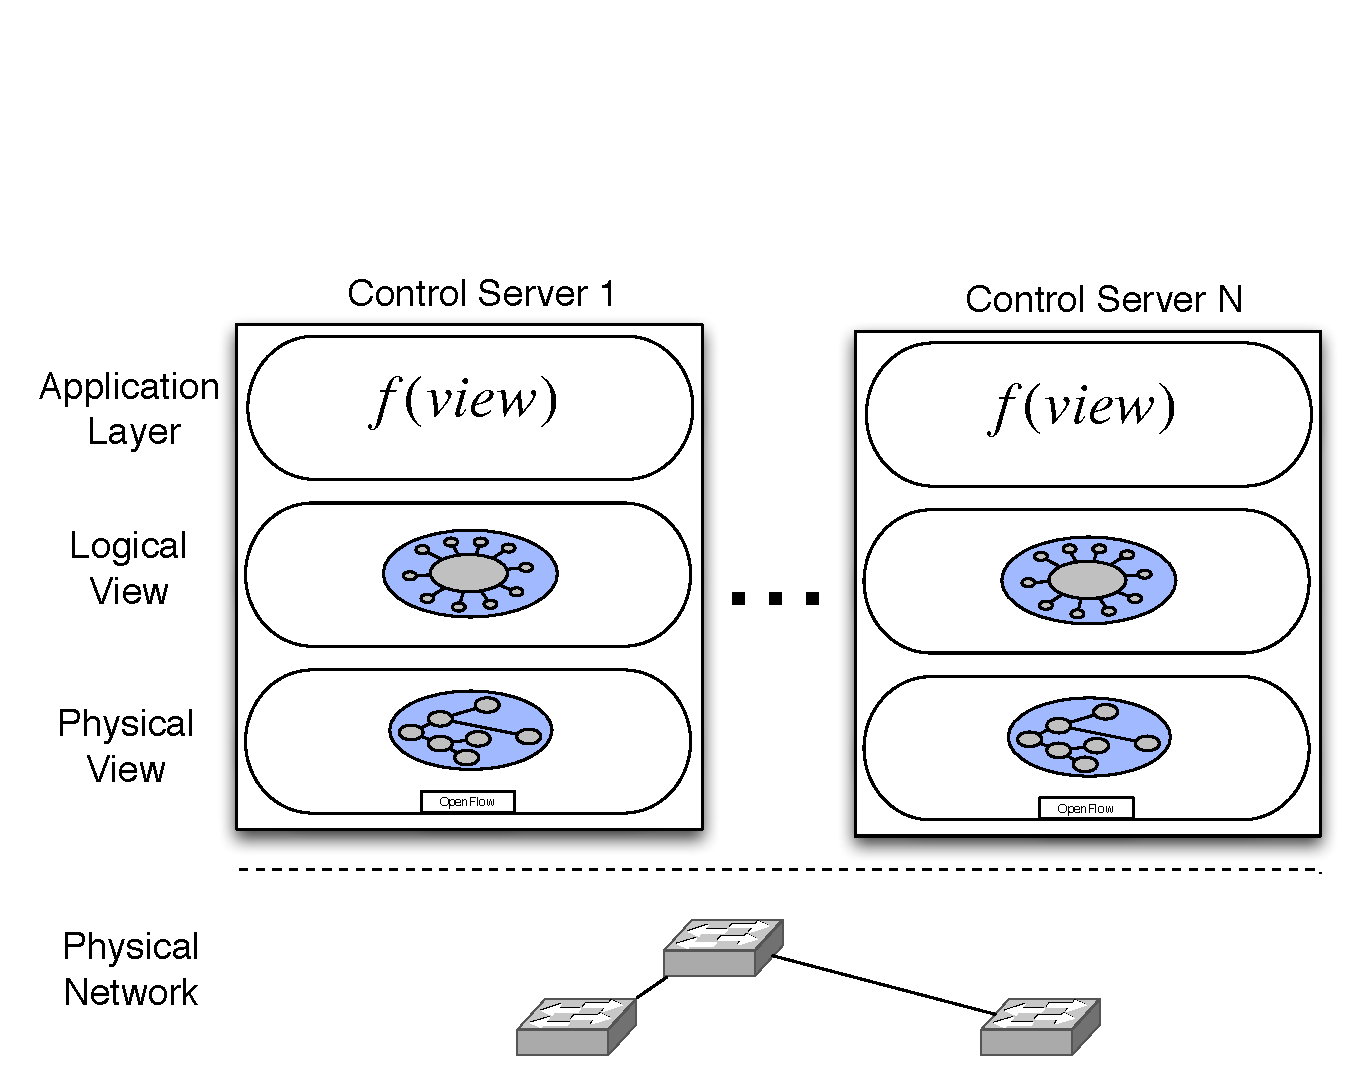
\includegraphics[width=3.25in]{../diagrams/architecture/SDN_Stack.pdf}
    \caption[]{\label{fig:basicarch} The SDN Software Architecture }
\end{figure}

\eat{
In this paper we focus on bugs in the virtualization and controller coordination
components of the SDN software stack. We focus on a \emph{proactive} mode of
operation where forwarding state updates are triggered by policy or topology
changes, not data-plane events.\footnote{It is possible to generalize our
approach to include inputs from the data-plane, subject to performance limitations.}
}

%We are primarily concerned with corner-case scenarios such as
%correlated hardware failures, which are the hardest to test {\it a priori}
%\andi{Check with our assumptions, i.e., uncorrelated external events}.
%Corner-case scenarios, while rare, cannot be ignored because of the distributed
%nature and large scale of production networks.
}
